\clearpage
\section{Large complementary intervals}
\label{sec:complement}

Throughout this report, $\alpha$ denotes the leading small-interval
power and $\beta$ the leading large-interval deficit power.
For the latter, $\beta_{\rm CFT}$ is the analytical prediction and
$\widehat\beta$ is the freely fitted exponent.

\subsection{Step 1: specify the interval and the observable}
The primaries and their lattice representatives are the same as in
Secs.~\ref{sec:construction} and \ref{sec:large-scales}.
Let $A=\{0,\ldots,\ell-1\}$ contain $\ell$ consecutive sites, and let
$B=\{\ell,\ldots,N-1\}$ be its complement on the periodic chain.
Define
\begin{equation}
 y=\frac{\ell}{N},\qquad x_B=1-y,\qquad
 \rho_a^B=\Tr_A\ket a\bra a,\qquad
 \bar\rho_{ab}^B=\frac{\rho_a^B+\rho_b^B}{2}.
 \label{eq:complement-geometry}
\end{equation}
Here $a,b$ label distinct primaries, $p=1/2$ is the mixing probability,
and $y$ always denotes the small complement fraction in this section.
The theory manuscript uses $y$ for a mixing probability in some formulas;
that manuscript variable is set to $1/2$ here. Its small parameter
$\epsilon=1-x$ is our $y$.
For each ordered pair we calculate
\begin{equation}
 D^B_{a\mid b}=\Tr\rho_a^B(\log\rho_a^B-\log\bar\rho_{ab}^B),
 \qquad \delta_{a\mid b}(y)=\log2-D^B_{a\mid b}.
 \label{eq:complement-deficit}
\end{equation}
All logarithms are natural. The two directions use the same incoherent
mixture; the source state changes. Positivity and
$\bar\rho_{ab}^B\geq\rho_a^B/2$ imply $0\leq D^B_{a\mid b}\leq\log2$.
The manuscript predicts $D^B_{a\mid b}\to\log2$ as $y\to0$.
The deficit resolves the approach to this limit more clearly than
$D^B_{a\mid b}$ alone.

The active mixture grid is Eq.~\eqref{eq:extended-grid}, with
$\ell=6,\ldots,10$. All models and all six directions use
$0<y\leq0.002$ for Ising or $0<y\leq0.005$ for the boson,
as in Eq.~\eqref{eq:common-fit-windows}. The boson window is prescribed;
its coefficient comparisons are in Appendix~\ref{sec:common-window-results}.
On the adopted large-interval windows, $F_2$ improves the leading coefficient over $F_1$ in 6 of six Ising directions and 4 of six compact-boson directions. Omitted-size prediction improves in 6 of six Ising directions and 2 of six compact-boson directions. The boson uses $0<y\leq0.005$; Appendix~\ref{sec:common-window-results} gives the full comparison.

The displayed range is $y\leq0.20$, or $x_B\geq0.80$.
Fits use $x_B\geq0.998$ for Ising and $x_B\geq0.995$ for the
boson. Counts are in Table~\ref{tab:scaling-grid}. Previously computed
$\ell=4,5,11,12$ observations remain archived and are excluded.
The overview figures and summary tables use the same fits as the
per-pair views in Sec.~\ref{sec:window-selection}.

\subsection{Step 2: replace the large matrix by a Gram matrix}
\label{sec:complement-gram}
Although $\rho_a^B$ acts on $2^{N-\ell}$ basis states, a pure global
state has Schmidt rank at most $2^\ell$ across this cut. A mixture of
two such states has rank at most $2^{\ell+1}$. To use this fact we need
both the individual matrices on $A$ and the transition matrix
\begin{equation}
 \rho_a^A=\Tr_B\ket a\bra a,\qquad
 T_{ab}^A=\Tr_B\ket a\bra b .
 \label{eq:complement-transition}
\end{equation}
The transition is generally neither Hermitian nor a density matrix.
It records how the two Schmidt supports overlap on $B$; the individual
$\rho_a^A,\rho_b^A$ do not determine that overlap.

For the derivation only, write
$\ket a=\sum_{u,v}X_a(v,u)\ket u_A\ket v_B$,
where $u$ and $v$ enumerate spin configurations.
Let $Z=(X_a,X_b)/\sqrt2$. Then
$ZZ^\dagger=\bar\rho_{ab}^B$, while its small Gram matrix is
\begin{equation}
 {\cal G}=Z^\dagger Z
 =\frac12\begin{pmatrix}
  (\rho_a^A)^T &(T_{ab}^A)^*\\
  (T_{ab}^A)^T&(\rho_b^A)^T
 \end{pmatrix}.
 \label{eq:complement-gram}
\end{equation}
The transpose and complex conjugation follow from assigning the $A$
configuration to the column of $X_a$; they must not be dropped.
The nonzero eigenvalues $\lambda_k$ of $\mathcal G$ are exactly those
of $\bar\rho_{ab}^B$. If $v_k$ is its normalized eigenvector, define
$P_a=\operatorname{diag}(\id_{2^\ell},0)$ and
$P_b=\operatorname{diag}(0,\id_{2^\ell})$.
The corresponding normalized large-space vector is
$w_k=Zv_k/\sqrt{\lambda_k}$.
Using $X_a=\sqrt2 ZE_a$, where $E_a$ embeds the first block, gives
$\bra{w_k}\rho_a^B\ket{w_k}=2\lambda_k v_k^\dagger P_a v_k$.
Purity equates the nonzero spectra of $\rho_a^A$ and $\rho_a^B$.
Therefore the complete entropy is
\begin{equation}
 D^B_{a\mid b}
 =\Tr(\rho_a^A\log\rho_a^A)
   -2\sum_{\lambda_k>0}\lambda_k
       (v_k^\dagger P_a v_k)\log\lambda_k .
 \label{eq:complement-entropy}
\end{equation}
Replace $P_a$ by $P_b$ and $\rho_a^A$ by $\rho_b^A$ for the other
direction. This form avoids division by small eigenvalues.
Multiplying $T_{ab}^A$ by one constant phase only conjugates
$\mathcal G$ by a block-diagonal unitary and leaves both entropies unchanged.

We diagonalize common quantum-number blocks on $B$. An Ising block
has parity $\mathfrak p_a(-1)^{|u|}$, with
$\mathfrak p_I=\mathfrak p_\varepsilon=1$,
$\mathfrak p_\sigma=-1$, and $|u|$ the number of occupied sites in $u$.
The scalar parity $\mathfrak p_a$ is distinct from the block projector $P_a$.
A boson block has $M_a-|u|$ occupied sites on $B$, where
$M_a$ is the total occupation in state $a$.
At $\ell=12$ the full Gram dimension is 8192; the largest symmetry
blocks are 4096 for Ising and 1716 for the boson pairs. We construct
each common-$B$ block directly, avoiding the full Gram allocation.
The production calculation constructs no state or matrix of dimension $2^{N-\ell}$.

For the new $\ell=11,12$ data, an additional numerical reduction
retains the occupied Schmidt vectors. In each local symmetry sector,
diagonalize $\rho_a^A$ and collect eigenvectors with eigenvalues
$\mu_{a,j}>\tau_s=10^{-16}$ in $U_a$; let
$\Lambda_a=\operatorname{diag}(\mu_{a,j})$ contain the retained values.
Use $U_b,\Lambda_b$ for the other state. Here these matrices collect
the retained vectors and values from all local sectors; the calculation
still diagonalizes each common-$B$ sector separately. With
$V=\operatorname{diag}(U_a^*,U_b^*)$, the projected Gram is
\begin{equation}
 {\cal G}_s=V^\dagger{\cal G}V
 =\frac12\begin{pmatrix}
 \Lambda_a &(U_a^\dagger T_{ab}^A U_b)^*\\
 (U_a^\dagger T_{ab}^A U_b)^T&\Lambda_b
 \end{pmatrix}.
 \label{eq:complement-support}
\end{equation}
Use the same source-weight formula in Eq.~\eqref{eq:complement-entropy},
with projectors onto the two retained blocks. The diagonal
$\Tr\rho_a^A\log\rho_a^A$ is evaluated from the corresponding
eigenvalues with the original entropy threshold $10^{-15}$.
This discards small Schmidt weights and is a numerical approximation.
We record $|1-\Tr\Lambda_a|$ and check the entropies against the full
Gram calculation and against $\tau_s=10^{-17},10^{-15}$ in
Sec.~\ref{sec:complement-extension-checks}. The $N=256$ benchmark
data themselves use the full Gram matrices.

\subsection{Step 3: obtain Ising transitions from anchored Gaussian states}
\label{sec:complement-ising}
Use the exact parity-resolved covariance $G_a$ of
Sec.~\ref{sec:large-ising} for each of $I,\sigma,\varepsilon$.
In our convention $\langle\gamma_r\gamma_s\rangle
=\delta_{rs}-i(G_a)_{rs}$ and $G_a^2=-\id$.
The $\gamma_r$ are Jordan--Wigner Majorana operators, with site zero
first. Distinct primaries are orthogonal, so a transition formula that
divides by $\langle b|a\rangle$ is singular. We remove that singularity
by acting on the bra state with a local Hermitian unitary:
\begin{equation}
 U_A=\begin{cases}
  \gamma_0=X_0,&\text{pairs containing }\sigma,\\
  i\gamma_0\gamma_1=-Z_0,& I,\varepsilon\text{ pair},
 \end{cases}
 \qquad \ket{b'}=U_A\ket b .
 \label{eq:complement-anchor}
\end{equation}
Here $X_0,Z_0$ are Pauli matrices on site zero.
The first choice changes parity; the second couples the two even
states. Both give a nonzero overlap with $\ket a$ on the tested grid.
They are computational devices and do not change the production
primary states.

Conjugation gives $G_{b'}=R G_bR^T$, where $R$ is diagonal with minus
signs at index $0$ for the first case or at $0,1$ for the second case,
and plus signs elsewhere. In the first case the true Majorana
reflection differs by an overall minus sign, which cancels in the covariance.
The Gaussian overlap and product rules
\cite{Bravyi,Surace} give, in our convention,
\begin{align}
 K&=\id-G_aG_{b'},&
 o&=|\langle b'|a\rangle|
   =2^{-N/2}\det(K)^{1/4},\nonumber\\
 Q&=(\id-iG_{b'})K^{-1}(\id-iG_a),&
 G_*&=i(Q-\id).
 \label{eq:complement-transition-covariance}
\end{align}
The inverse denotes a linear solve. We evaluate
$\log o=\tfrac14\sum_j\log s_j(K)-\tfrac N2\log2$
from the positive singular values $s_j(K)$, avoiding a large determinant.
The matrix $G_*$ is complex antisymmetric and describes the trace-one
operator $\ket a\bra{b'}/\langle b'|a\rangle$.
It need not describe a physical density matrix.

Restrict $G_*$ to its first $2\ell$ Majoranas. For any complex
antisymmetric matrix $H$ on those modes define the operator
\begin{equation}
 {\cal R}(H)=2^{-\ell}
   \sum_{\substack{S\subset\{0,\ldots,2\ell-1\}\\ |S|\ {\rm even}}}
   i^{|S|/2}\operatorname{Pf}(H_S)
   \prod_{r\in S}^{\longrightarrow}\gamma_r ,
 \qquad \operatorname{Pf}(H_\varnothing)=1 .
 \label{eq:complement-wick}
\end{equation}
$H_S$ is the principal submatrix on $S$, the product is in increasing
index order, and $\operatorname{Pf}$ denotes the Pfaffian introduced in
Sec.~\ref{sec:boson-contraction}. This is Wick's theorem expressed in
the Majorana operator basis. Undoing the local anchor gives
\begin{equation}
 T_{ab}^A=o\,{\cal R}((G_*)_A)U_A
 \quad\text{up to one overall phase}.
 \label{eq:complement-ising-transition}
\end{equation}
The code evaluates all principal Pfaffians recursively and converts
the Pauli-string coefficients to matrix entries with a Walsh transform.
It requires $O(\ell^2 4^\ell)$ local work and a $2N$-dimensional
covariance solve, without a full-chain wavefunction.
For the added diagonal matrices at $\ell=12$, the same reconstruction
gives $\rho_a^A={\cal R}((G_a)_A)$. It avoids forming and rotating
all 24 dense Majorana matrices; its reduction to $\ell=10$ is checked
against the existing Schur-based diagonal matrices.
The anchor and this reconstruction are project adaptations of the
published Gaussian identities. Their explicit-wavefunction checks are
reported in Sec.~\ref{sec:complement-checks}.

\subsection{Step 4: contract different boson occupation sectors exactly}
\label{sec:complement-boson}
The same conformal-block/Jastrow amplitudes of
Eq.~\eqref{eq:pf-amplitude} are used, with endpoint $W=10^8$.
To distinguish charge labels from state names, denote ket charges by
$(a_1,b_1)$ and bra charges by $(a_2,b_2)$, with
$(0,0),(1,1),(3,1)$ representing $00,ss,3s,s$.
Their occupied-site counts are $M_i=(N-a_i-b_i)/2$.
Let $U,V\subset A$ be the occupied sites in the ket and bra configurations;
$Y\subset B$ is their common occupied environment. A transition element
can be nonzero only when
\begin{equation}
 m=M_1-|U|=M_2-|V|,\qquad 0\leq m\leq N-\ell .
 \label{eq:complement-charge-selection}
\end{equation}
Thus different occupation numbers of the global primaries are fully
compatible with a nonzero transition on $A$.

Set $z_j=e^{2\pi i j/N}$, $g_i(z)=(1-z/W)^{b_i}$,
and define the unnormalized local polynomial
\begin{equation}
 L_i(U)=\prod_{j\in U}z_j^{a_i+1}g_i(z_j)
        \prod_{\substack{j<k\\j,k\in U}}(z_j-z_k)^2 .
 \label{eq:complement-local-boson}
\end{equation}
Splitting the full occupied set into $U\cup Y$ in the ket and
$V\cup Y$ in the bra, and using
$\overline{z_i-z_j}=-(z_i-z_j)/(z_i z_j)$, yields
\begin{align}
 (T_{12}^A)_{UV}
 &=\frac{L_1(U)\overline{L_2(V)}}{\sqrt{{\cal Z}_1{\cal Z}_2}}
       \prod_{j\in V}z_j^{-2m}\ {\cal E}_{UV},\nonumber\\
 {\cal E}_{UV}
 &=\sum_{\substack{Y\subset B\\|Y|=m}}
   \prod_{\substack{i<j\\i,j\in Y}}(z_i-z_j)^4
   \prod_{i\in Y}\left[
       w(z_i)\prod_{j\in A}(z_j-z_i)^{2\nu_j}\right],\nonumber\\
 \nu_j&=\mathbf1_{j\in U}+\mathbf1_{j\in V},\nonumber\\
 w(z)&=z^\kappa g_1(z)\overline{g_2(z)},\qquad
 \kappa=a_1-a_2-2M_2+2 .
 \label{eq:complement-environment}
\end{align}
Here $\mathcal Z_i$ is the full norm sum of state $i$.
The key identity is $2m+\sum_j\nu_j=M_1+M_2=:d$:
the moment-matrix dimension $d$ is independent of $U,V$.

To evaluate the environment sum, introduce the column
$f(z)=(1,z,\ldots,z^{d-1})^T$ and its derivative $f'(z)$.
The skew moment matrix on the environment is
\begin{equation}
 D_B=\sum_{j\in B}w(z_j)
       [f(z_j)f'(z_j)^T-f'(z_j)f(z_j)^T].
 \label{eq:complement-cross-moment}
\end{equation}
At each site $j\in A$, include no column if $\nu_j=0$,
$f(z_j)$ if $\nu_j=1$, and the two columns $f(z_j),f'(z_j)$
if $\nu_j=2$. Put these columns, in site order, in $E_{UV}$.
With $q=\sum_j\nu_j$ and
$\Delta_{\rm ext}=\prod_{i<j\in A}(z_j-z_i)^{\nu_i\nu_j}$,
the discrete confluent-Vandermonde identity gives
\begin{equation}
 {\cal E}_{UV}=
 \frac{(-1)^{q(q-1)/2}}{\Delta_{\rm ext}}\,
 \operatorname{Pf}
 \begin{pmatrix}D_B&E_{UV}\\-E_{UV}^T&0\end{pmatrix}.
 \label{eq:complement-bordered-pf}
\end{equation}
This follows by expanding the moment Pfaffian over distinct environment
sites. The confluent determinant contains their fourth-power Vandermonde,
the external factor $\Delta_{\rm ext}$, and the cross factors in
Eq.~\eqref{eq:complement-environment}. It extends the norm-sum construction
of St\'ephan and Pollmann \cite{Stephan} to a bra and ket with different
charges. It is an exact contraction of the interacting spin wavefunction.

Computing a new $d$-dimensional Pfaffian for every $U,V$ would waste
work. We instead use full-circle root-of-unity moments, remove the
$\ell$ sites of $A$ by a rank-$2\ell$ update, and cache the resulting
small Pfaffian minors. Odd $d$ and singular even cross moments require
the exact border/regularizer construction in
Sec.~\ref{sec:complement-pf-details}. All large-$N$ moment work then
uses sparse matrices; the final minors have at most $2\ell+1$ indices.
Through $N=256$ we evaluate the cancellation-prone moment algebra at 100 decimal digits
before converting $T_{12}^A$ to double precision.

\subsection{Step 5: test leading and next powers from CFT}
\label{sec:complement-theory}
The analytical source is \texttt{manuscript\_theory/main3.tex}
\cite{theoryLarge}. Its compiled \texttt{main.pdf} is an older version
without the worked examples used here. In the mixing operator product
expansion, let $\Delta$ be the lowest exchanged scaling dimension and
$c_{ab}$ its normalized coefficient. At $p=1/2$ the leading deficit is
\begin{equation}
 \delta_{a\mid b}(y)=B_{ab}y^{\beta_{\rm CFT}}+\cdots,\qquad
 \beta_{\rm CFT}=2\Delta,\qquad
 B_{ab}=\pi^{2\Delta}|c_{ab}|^2
 \frac{\sqrt\pi\,\Gamma(1+\Delta)}{4\Gamma(3/2+\Delta)}.
 \label{eq:complement-leading}
\end{equation}
$\Gamma$ is Euler's gamma function. In particular, $B_{ab}$ includes
$\pi^{\beta_{\rm CFT}}$. Each leading coefficient is shared by the
two directions; their higher-order coefficients need not coincide.
\begin{table}[htbp]\centering\small
\begin{tabular}{llccc}\toprule
CFT & Pair (both directions) & $\beta_{\rm CFT}$ & $B_{ab}$ & Next power\\\midrule
Ising & $I,\sigma$ & $1/4$ & $\pi^{3/4}\Gamma(9/8)/[4\Gamma(13/8)]$ & $1/2$\\
Ising & $I,\eps$ & $2$ & $\pi^2/3$ & $4$\\
Ising & $\sigma,\eps$ & $1/4$ & $\pi^{3/4}\Gamma(9/8)/[16\Gamma(13/8)]$ & $1/2$\\
Boson & $00,ss$ & $1$ & $\pi^2/8$ & $2$\\
Boson & $00,3s,s$ & $5$ & $5\pi^6/64$ & $6$\\
Boson & $ss,3s,s$ & $2$ & $\pi^2/3$ & $3$ (allowed)\\\bottomrule
\end{tabular}
\caption{Leading large-interval amplitudes multiplying $y^\beta$ and
next powers used in $F_2$, at $p=1/2$ and $s=1/\sqrt2$.
The Ising spin--energy channel includes $|c_{\sigma\eps}|^2=1/4$.
For boson charge codes $(a_i,b_i)$,
$\Delta=[(a_1-a_2)^2+(b_1-b_2)^2]/4$ and $|c_{ab}|=1$.
The last next power follows from the manuscript's general three-point
sector rather than a separately evaluated example; its coefficient may
vanish. No next-order coefficient is supplied or derived here.}
\label{tab:complement-theory}
\end{table}

The manuscript's Ising examples explicitly identify four-spin terms
of order $y^{1/2}$ and later two-spin--energy terms of order $y^{5/4}$;
the first correction retained in $F_2$ is $y^{1/2}$. The identity--energy
example specifies a remainder of order $y^4$. The boson vacuum examples
specify orders $y^2$ and $y^6$. For the remaining boson pair, the general
subsection ``Three point function'' contains powers
$2\Delta_{L'}+\Delta_L$: the exchanged vertex has $\Delta_{L'}=1$
and a current has $\Delta_L=1$, giving the candidate power three.
This identifies an allowed sector, not a proved nonzero total
coefficient after replica continuation. We consequently interpret
that pair's $F_2$ as a test of the next allowed power. This qualification
also prevents an $O(y^r)$ remainder from being mistaken for a known
coefficient. No universal increment of two is imposed for large intervals.

\begin{equation}
 F_{\rm free}(y)=Cy^{\widehat\beta},\qquad
 F_1(y)=c_0y^{\beta_{\rm CFT}},\qquad
 F_2(y)=c_0y^{\beta_{\rm CFT}}+c_1y^{\beta_1}.
 \label{eq:complement-fit}
\end{equation}
Here $\beta_1$ is the next power in Table~\ref{tab:complement-theory}.
Only the exponents of $F_1,F_2$ are imposed; all their coefficients
are fitted separately in each direction. ``CFT leading'' always means
$B_{ab}y^{\beta_{\rm CFT}}$, with neither parameter fitted.
For completeness, the one-term solution is
\begin{equation}
 c_0=\frac{\sum_i y_i^{\beta_{\rm CFT}}\delta_i}
                 {\sum_i y_i^{2\beta_{\rm CFT}}}.
 \label{eq:complement-fixed-fit}
\end{equation}
The fits use the CFT-wide windows in Eq.~\eqref{eq:common-fit-windows}:
$y\leq0.002$ for Ising and $y\leq0.005$ for the boson. Every
direction uses the same window as its reverse. Figures show data
through $y\leq0.20$, with fitting-window zooms in the per-pair views.
The objective, coefficient convention, residuals and size cross-validation
are exactly Eqs.~\eqref{eq:objective}, \eqref{eq:metrics} and \eqref{eq:cv}.
\begin{equation}
 R_i=100[\delta_i-M(y_i)]/\delta_i,\qquad
 \eta_\beta=100(\widehat\beta/\beta_{\rm CFT}-1).
 \label{eq:complement-fit-metrics}
\end{equation}
\begin{equation}
 \mathrm{CVRMSE}=\sqrt{m^{-1}\sum_i[\delta_i-M^{(-N_i)}(y_i)]^2}.
 \label{eq:complement-cv}
\end{equation}
The residual sign in the entropy $D^B=\log2-\delta$ is opposite to
the deficit residual. Tables in Appendix~\ref{sec:complement-checks}
separate Free, $F_1$, $F_2$ and CFT rows for all twelve directions.
\subsection{Results}
\label{sec:complement-results}
Ising full-window free-exponent deviations range from $-0.074\%$ to $+5.861\%$. $F_2$ improves size-holdout RMSE over $F_1$ in 6 of six directions. These statements use the prescribed fitting window and the sample-count requirements in Appendix~\ref{sec:window-comparison}.\par
Compact-boson full-window free-exponent deviations range from $-0.438\%$ to $-0.074\%$. $F_2$ improves size-holdout RMSE over $F_1$ in 2 of six directions. These statements use the prescribed fitting window and the sample-count requirements in Appendix~\ref{sec:window-comparison}.\par

\begin{figure}[p]\centering
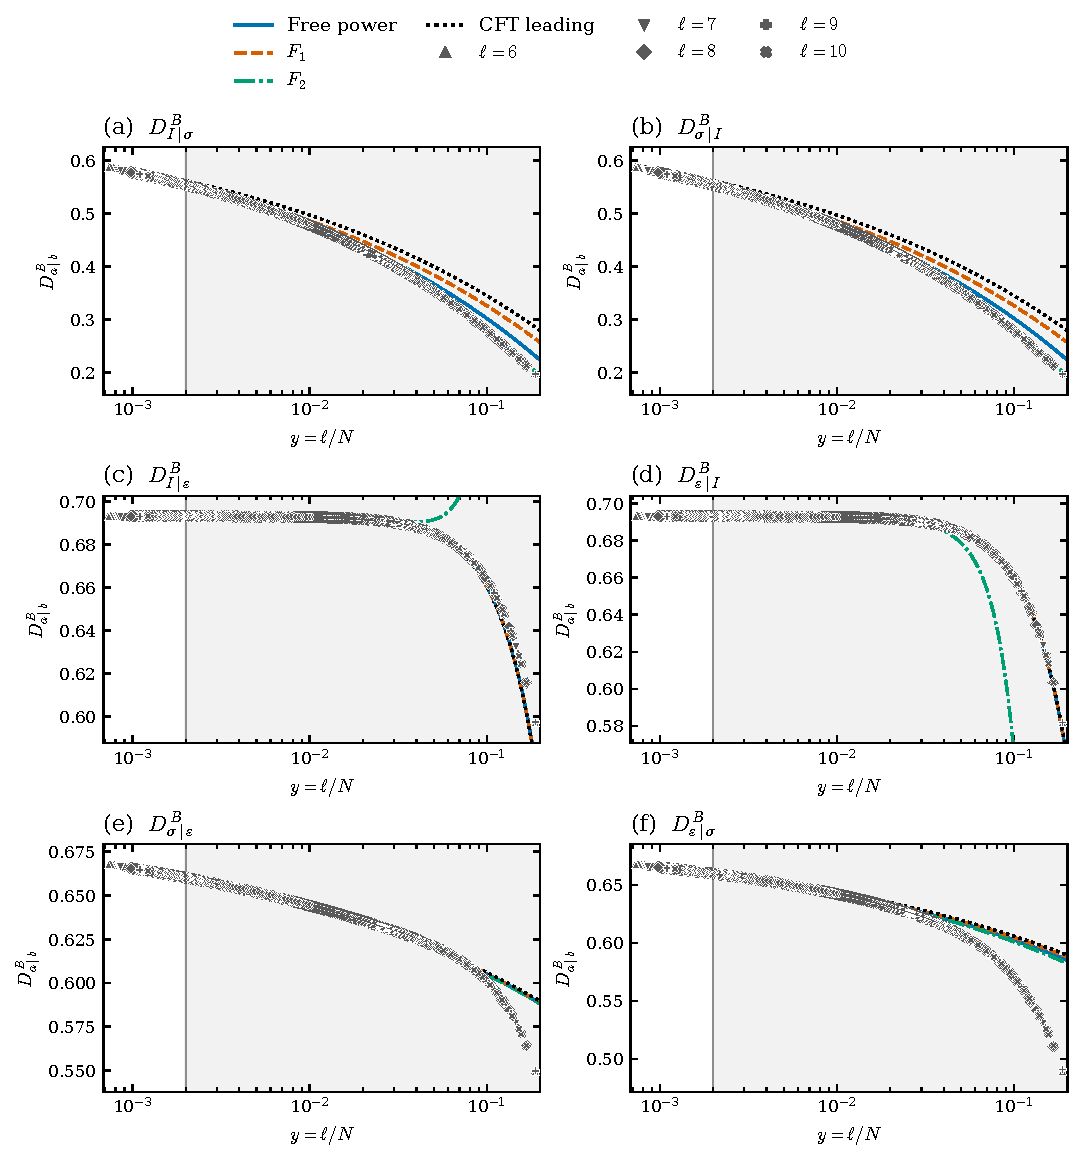
\includegraphics[width=.88\linewidth]{../figs/ising_large_entropy.pdf}
\caption{The ordinate is $D^B=\log2-\delta$, on a linear scale; tick labels give its value directly, without an additive offset. The fraction axis is logarithmic. Ising mixtures at $p=1/2$, $\ell=6,7,8,9,10$, and the chain-size set in Eq.~\eqref{eq:extended-grid}, with $32\leq N\leq8192$. There are 1645 displayed geometries per direction at $y\leq0.2$, of which 260 satisfy $y\leq0.002$ and enter every fit. Marker shape identifies $\ell$; the vertical boundary and gray shading mark the fitting cutoff and excluded data. The periodic Ising Hamiltonian is $H=-\sum_jX_jX_{j+1}-\sum_jZ_j$; primaries use exact fermionic covariances, including the odd Ramond ground state for $\sigma$. Natural logarithms apply. Added sizes use the direct entropy remainder in Sec.~\ref{sec:stable-entropy}, with support cutoff $10^{-15}$. Blue solid is the free-power fit (two fitted parameters), orange dashed is $F_1$ (one), green dash--dot is $F_2$ (two), and black dotted is the analytical CFT leading term (zero). Powers and amplitudes use Eqs.~\eqref{eq:fit} and \eqref{eq:complement-fit}; all coefficients include powers of $\pi$. Fits minimize unweighted squared residuals in $\delta$. These curves use \texttt{scaling\_fit\_summary.csv}. The identical fits in Tables~\ref{tab:ising-large-parameters} and \ref{tab:ising-large-metrics} also have per-pair full-range and fitting-window views in Sec.~\ref{sec:pair-large_ising}.}
\label{fig:ising-complement-entropy}
\end{figure}

\begin{figure}[p]\centering
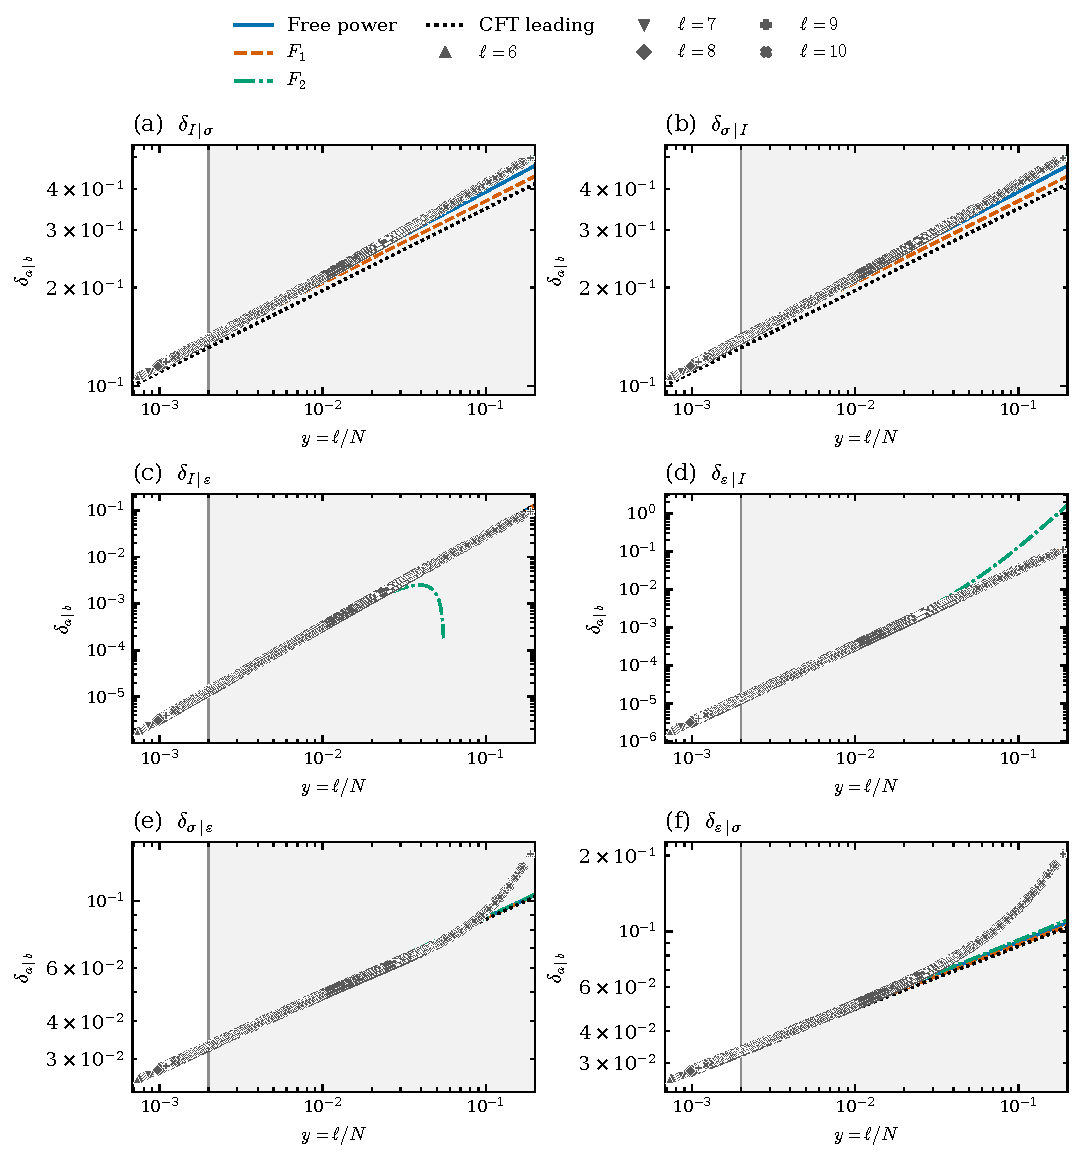
\includegraphics[width=.88\linewidth]{../figs/ising_large_value.pdf}
\caption{Both axes are logarithmic. Nonpositive values of an extrapolated truncated curve are omitted only from this logarithmic panel, while residual panels retain their predictions. Ising mixtures at $p=1/2$, $\ell=6,7,8,9,10$, and the chain-size set in Eq.~\eqref{eq:extended-grid}, with $32\leq N\leq8192$. There are 1645 displayed geometries per direction at $y\leq0.2$, of which 260 satisfy $y\leq0.002$ and enter every fit. Marker shape identifies $\ell$; the vertical boundary and gray shading mark the fitting cutoff and excluded data. The periodic Ising Hamiltonian is $H=-\sum_jX_jX_{j+1}-\sum_jZ_j$; primaries use exact fermionic covariances, including the odd Ramond ground state for $\sigma$. Natural logarithms apply. Added sizes use the direct entropy remainder in Sec.~\ref{sec:stable-entropy}, with support cutoff $10^{-15}$. Blue solid is the free-power fit (two fitted parameters), orange dashed is $F_1$ (one), green dash--dot is $F_2$ (two), and black dotted is the analytical CFT leading term (zero). Powers and amplitudes use Eqs.~\eqref{eq:fit} and \eqref{eq:complement-fit}; all coefficients include powers of $\pi$. Fits minimize unweighted squared residuals in $\delta$. These curves use \texttt{scaling\_fit\_summary.csv}. The identical fits in Tables~\ref{tab:ising-large-parameters} and \ref{tab:ising-large-metrics} also have per-pair full-range and fitting-window views in Sec.~\ref{sec:pair-large_ising}.}
\label{fig:ising-complement-deficit}
\end{figure}

\begin{figure}[p]\centering
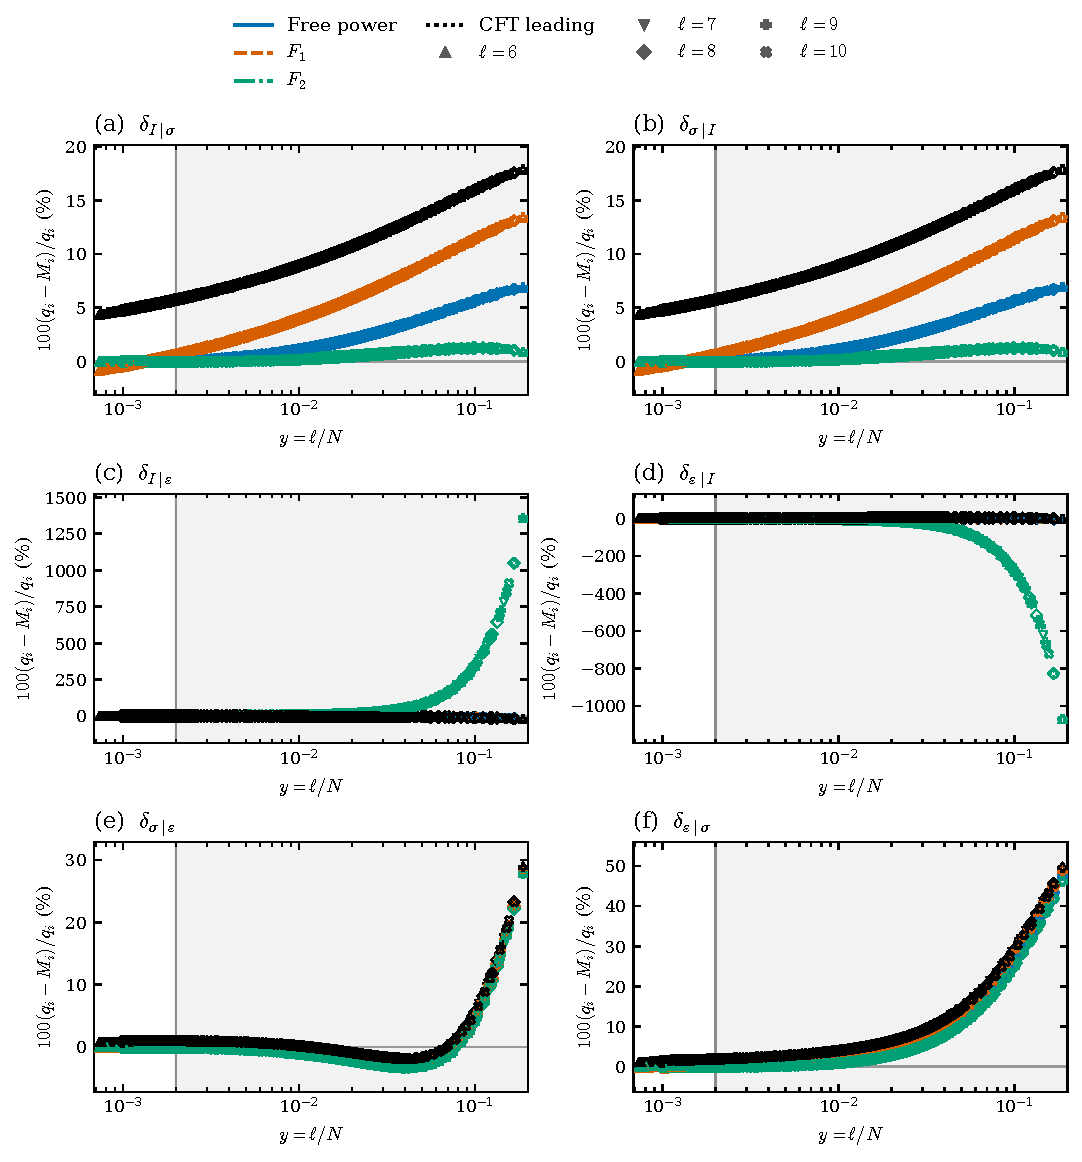
\includegraphics[width=.88\linewidth]{../figs/ising_large_residual.pdf}
\caption{The ordinate is $100(q_i-M_i)/q_i$ percent, with $q_i=D^A_i$ for a small interval and $q_i=\delta_i$ for a large interval; the horizontal zero line aids comparison. All four models have residual markers, colored as their curves. The residual ordinate is linear; the fraction axis is logarithmic. Ising mixtures at $p=1/2$, $\ell=6,7,8,9,10$, and the chain-size set in Eq.~\eqref{eq:extended-grid}, with $32\leq N\leq8192$. There are 1645 displayed geometries per direction at $y\leq0.2$, of which 260 satisfy $y\leq0.002$ and enter every fit. Marker shape identifies $\ell$; the vertical boundary and gray shading mark the fitting cutoff and excluded data. The periodic Ising Hamiltonian is $H=-\sum_jX_jX_{j+1}-\sum_jZ_j$; primaries use exact fermionic covariances, including the odd Ramond ground state for $\sigma$. Natural logarithms apply. Added sizes use the direct entropy remainder in Sec.~\ref{sec:stable-entropy}, with support cutoff $10^{-15}$. Blue solid is the free-power fit (two fitted parameters), orange dashed is $F_1$ (one), green dash--dot is $F_2$ (two), and black dotted is the analytical CFT leading term (zero). Powers and amplitudes use Eqs.~\eqref{eq:fit} and \eqref{eq:complement-fit}; all coefficients include powers of $\pi$. Fits minimize unweighted squared residuals in $\delta$. These curves use \texttt{scaling\_fit\_summary.csv}. The identical fits in Tables~\ref{tab:ising-large-parameters} and \ref{tab:ising-large-metrics} also have per-pair full-range and fitting-window views in Sec.~\ref{sec:pair-large_ising}.}
\label{fig:ising-complement-residuals}
\end{figure}

\begin{figure}[p]\centering
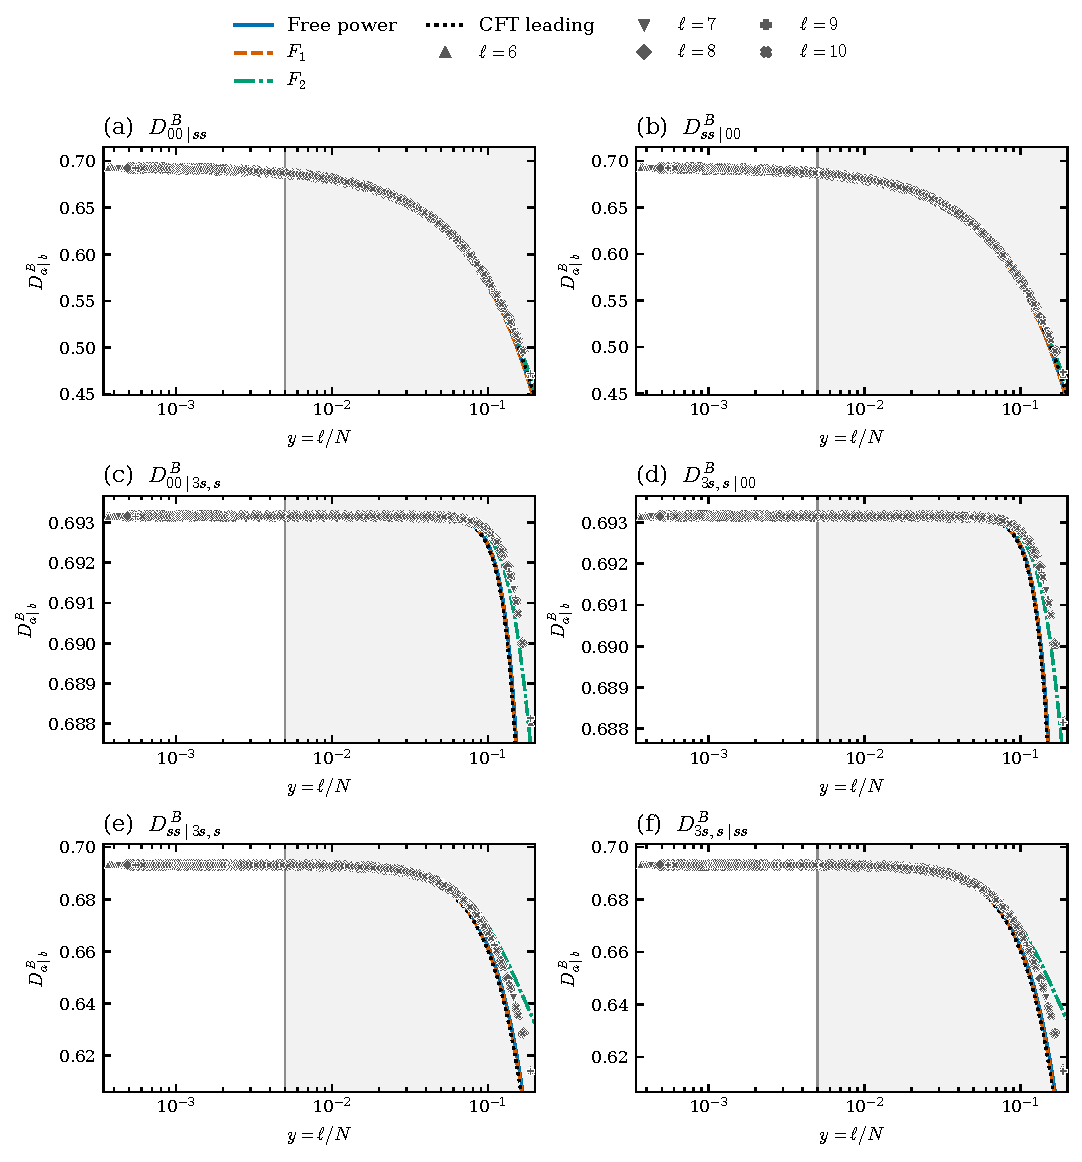
\includegraphics[width=.88\linewidth]{../figs/boson_large_entropy.pdf}
\caption{The ordinate is $D^B=\log2-\delta$, on a linear scale; tick labels give its value directly, without an additive offset. The fraction axis is logarithmic. Compact-boson mixtures at $p=1/2$, $\ell=6,7,8,9,10$, and the chain-size set in Eq.~\eqref{eq:extended-grid}, with $32\leq N\leq16384$. There are 625 displayed geometries per direction at $y\leq0.2$, of which 317 satisfy $y\leq0.005$ and enter every fit. Marker shape identifies $\ell$; the vertical boundary and gray shading mark the fitting cutoff and excluded data. The boson uses $s=1/\sqrt2$, $q=2$, charge codes $(0,0),(1,1),(3,1)$, $z_j=e^{2\pi i j/N}$, $w_1=0$, and $W=10^8$; moment algebra uses 100 digits through $N=256$ and 120 digits at the added sizes. Natural logarithms apply. Added sizes use the direct entropy remainder in Sec.~\ref{sec:stable-entropy}, with support cutoff $10^{-15}$. Blue solid is the free-power fit (two fitted parameters), orange dashed is $F_1$ (one), green dash--dot is $F_2$ (two), and black dotted is the analytical CFT leading term (zero). Powers and amplitudes use Eqs.~\eqref{eq:fit} and \eqref{eq:complement-fit}; all coefficients include powers of $\pi$. Fits minimize unweighted squared residuals in $\delta$. These curves use \texttt{scaling\_fit\_summary.csv}. The identical fits in Tables~\ref{tab:boson-large-parameters} and \ref{tab:boson-large-metrics} also have per-pair full-range and fitting-window views in Sec.~\ref{sec:pair-large_boson}.}
\label{fig:boson-complement-entropy}
\end{figure}

\begin{figure}[p]\centering
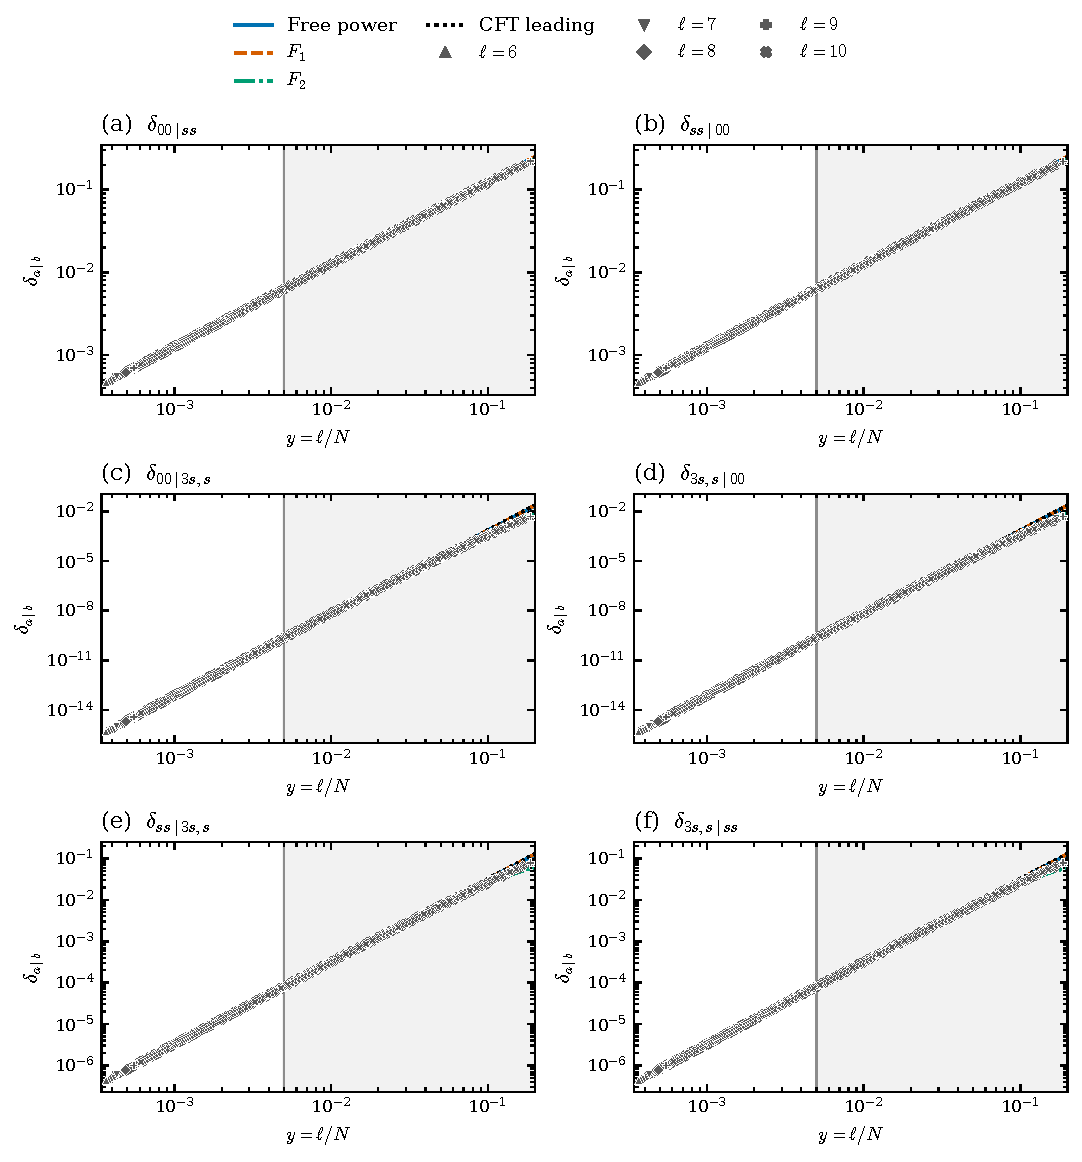
\includegraphics[width=.88\linewidth]{../figs/boson_large_value.pdf}
\caption{Both axes are logarithmic. Nonpositive values of an extrapolated truncated curve are omitted only from this logarithmic panel, while residual panels retain their predictions. Compact-boson mixtures at $p=1/2$, $\ell=6,7,8,9,10$, and the chain-size set in Eq.~\eqref{eq:extended-grid}, with $32\leq N\leq16384$. There are 625 displayed geometries per direction at $y\leq0.2$, of which 317 satisfy $y\leq0.005$ and enter every fit. Marker shape identifies $\ell$; the vertical boundary and gray shading mark the fitting cutoff and excluded data. The boson uses $s=1/\sqrt2$, $q=2$, charge codes $(0,0),(1,1),(3,1)$, $z_j=e^{2\pi i j/N}$, $w_1=0$, and $W=10^8$; moment algebra uses 100 digits through $N=256$ and 120 digits at the added sizes. Natural logarithms apply. Added sizes use the direct entropy remainder in Sec.~\ref{sec:stable-entropy}, with support cutoff $10^{-15}$. Blue solid is the free-power fit (two fitted parameters), orange dashed is $F_1$ (one), green dash--dot is $F_2$ (two), and black dotted is the analytical CFT leading term (zero). Powers and amplitudes use Eqs.~\eqref{eq:fit} and \eqref{eq:complement-fit}; all coefficients include powers of $\pi$. Fits minimize unweighted squared residuals in $\delta$. These curves use \texttt{scaling\_fit\_summary.csv}. The identical fits in Tables~\ref{tab:boson-large-parameters} and \ref{tab:boson-large-metrics} also have per-pair full-range and fitting-window views in Sec.~\ref{sec:pair-large_boson}.}
\label{fig:boson-complement-deficit}
\end{figure}

\begin{figure}[p]\centering
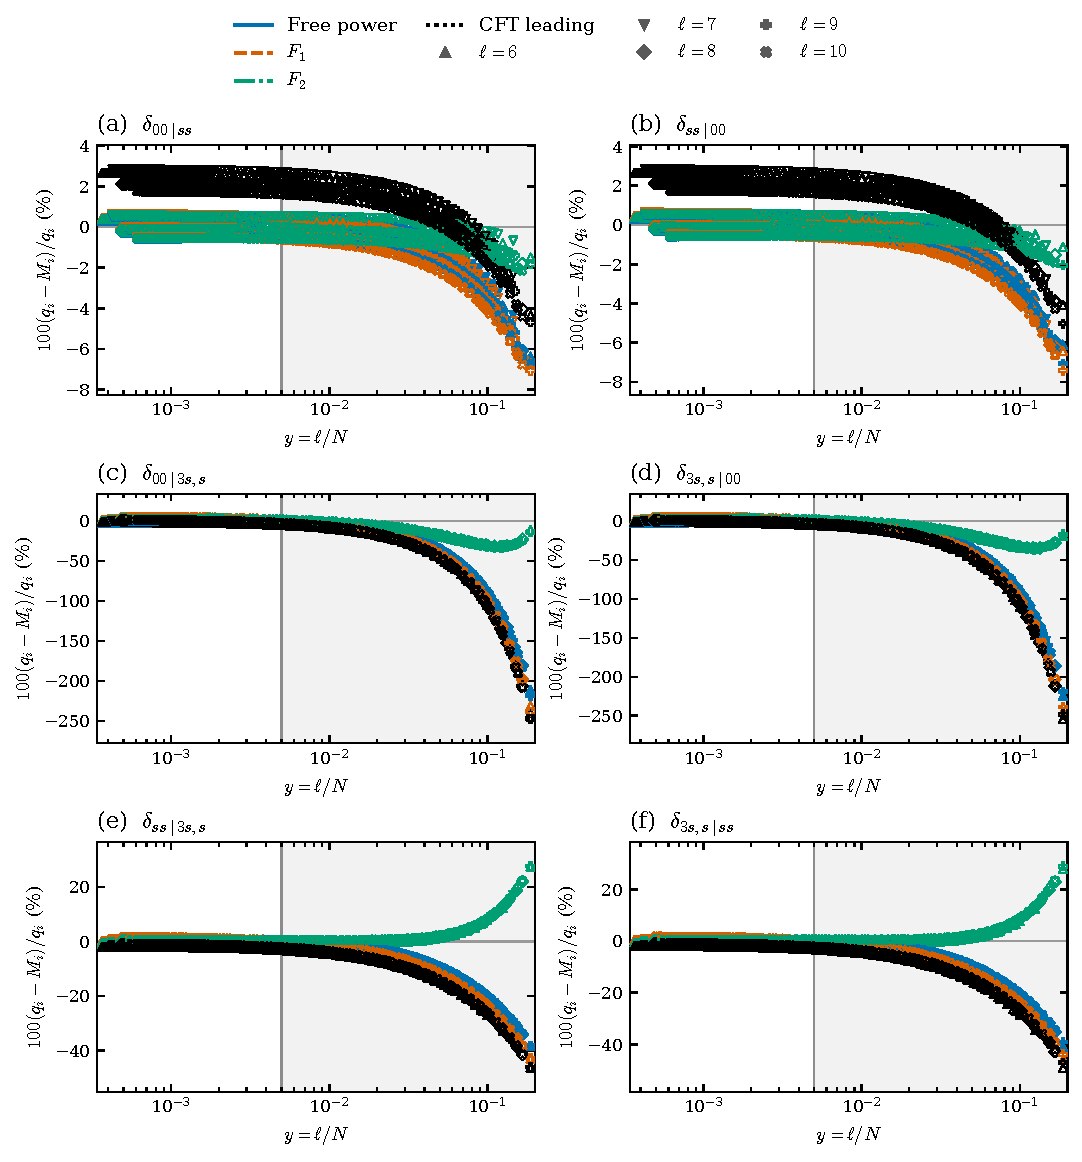
\includegraphics[width=.88\linewidth]{../figs/boson_large_residual.pdf}
\caption{The ordinate is $100(q_i-M_i)/q_i$ percent, with $q_i=D^A_i$ for a small interval and $q_i=\delta_i$ for a large interval; the horizontal zero line aids comparison. All four models have residual markers, colored as their curves. The residual ordinate is linear; the fraction axis is logarithmic. Compact-boson mixtures at $p=1/2$, $\ell=6,7,8,9,10$, and the chain-size set in Eq.~\eqref{eq:extended-grid}, with $32\leq N\leq16384$. There are 625 displayed geometries per direction at $y\leq0.2$, of which 317 satisfy $y\leq0.005$ and enter every fit. Marker shape identifies $\ell$; the vertical boundary and gray shading mark the fitting cutoff and excluded data. The boson uses $s=1/\sqrt2$, $q=2$, charge codes $(0,0),(1,1),(3,1)$, $z_j=e^{2\pi i j/N}$, $w_1=0$, and $W=10^8$; moment algebra uses 100 digits through $N=256$ and 120 digits at the added sizes. Natural logarithms apply. Added sizes use the direct entropy remainder in Sec.~\ref{sec:stable-entropy}, with support cutoff $10^{-15}$. Blue solid is the free-power fit (two fitted parameters), orange dashed is $F_1$ (one), green dash--dot is $F_2$ (two), and black dotted is the analytical CFT leading term (zero). Powers and amplitudes use Eqs.~\eqref{eq:fit} and \eqref{eq:complement-fit}; all coefficients include powers of $\pi$. Fits minimize unweighted squared residuals in $\delta$. These curves use \texttt{scaling\_fit\_summary.csv}. The identical fits in Tables~\ref{tab:boson-large-parameters} and \ref{tab:boson-large-metrics} also have per-pair full-range and fitting-window views in Sec.~\ref{sec:pair-large_boson}.}
\label{fig:boson-complement-residuals}
\end{figure}


